\section{Design}
\label{sec:design}

Section~\ref{sec:background} showed that putting a seed next to the neighbors a search actually follows can raise QPS, but storing every node's full neighborhood is too large.
\textsc{NeighborCache} keeps a smaller version of that idea on SSD: only some seeds, and beside each seed only its hot neighbors.
Heats come from live search.
The base DiskANN index and search algorithm stay unchanged.
Figure~\ref{fig:design_overview} is the layout: DRAM holds the N-cache, M-cache, heaps, and commit queue; SSD holds the D-cache.

\begin{figure*}[t]
  \centering
  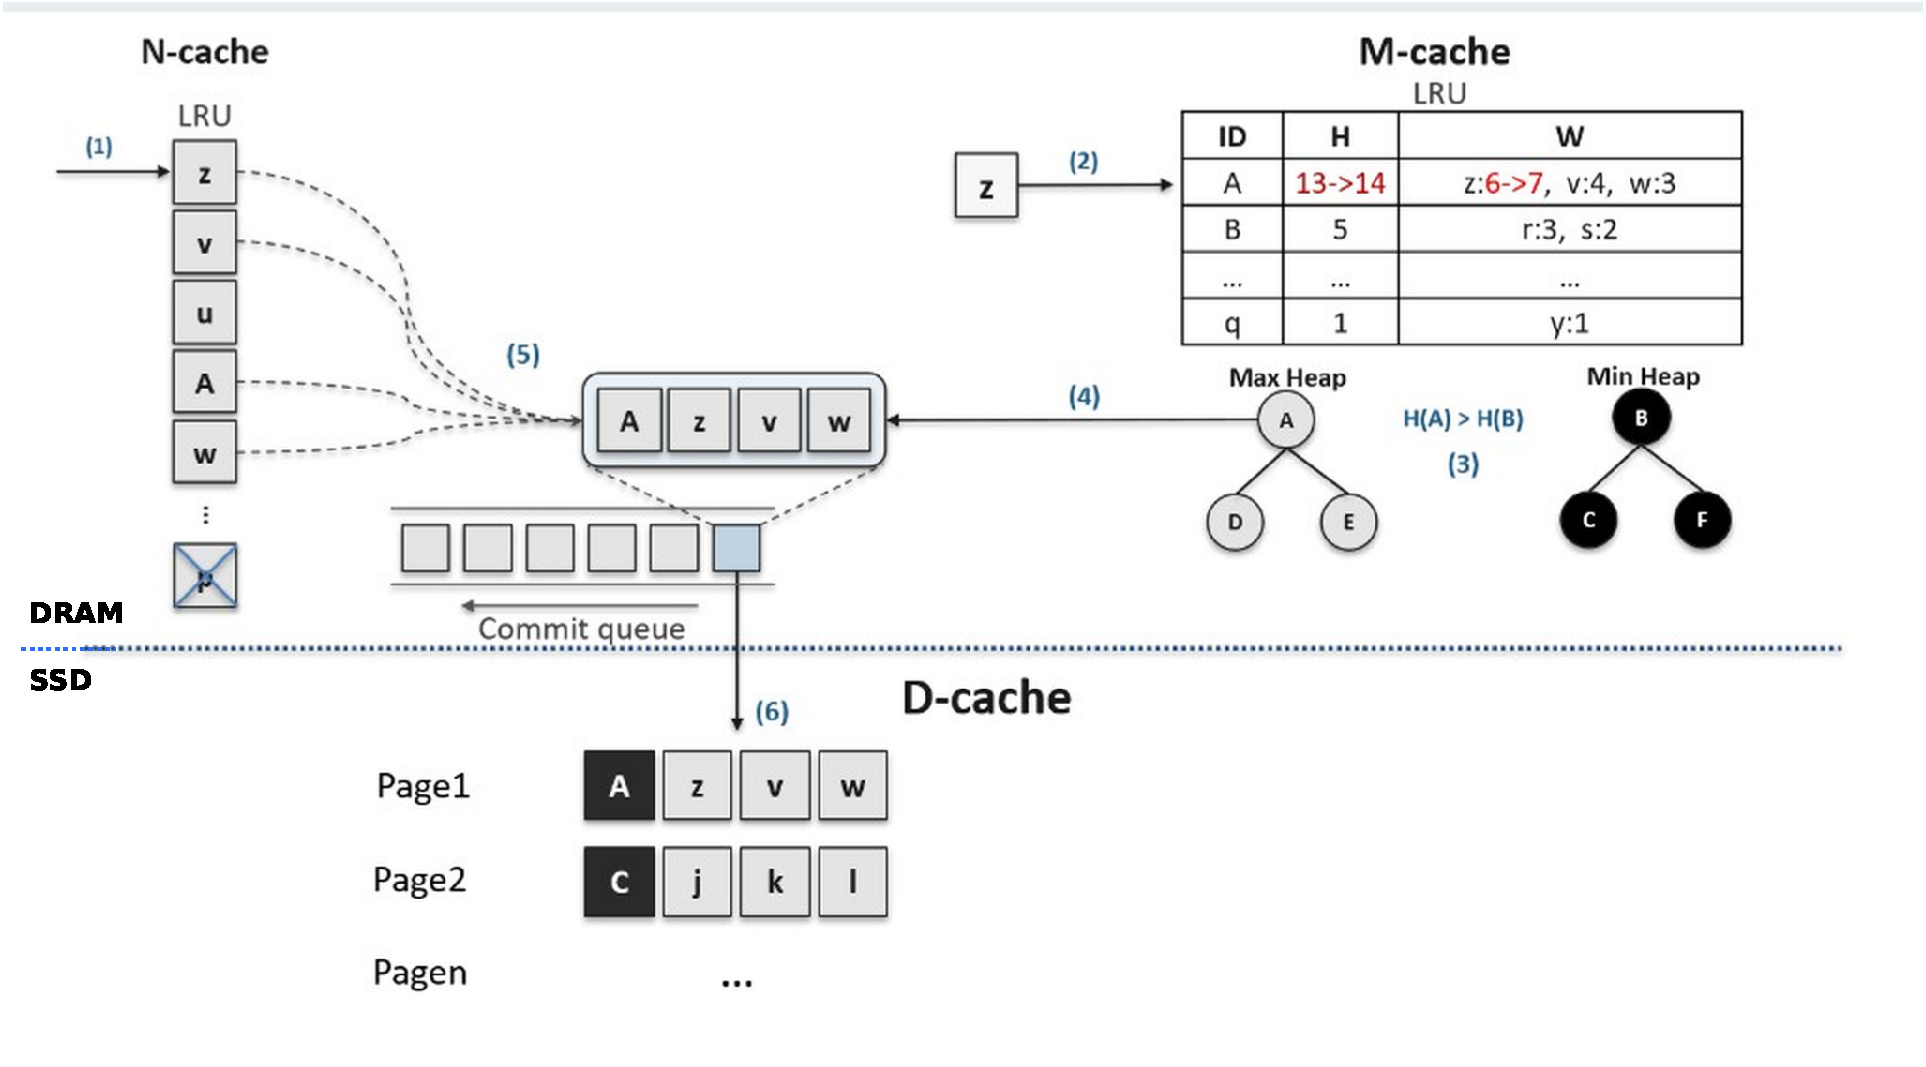
\includegraphics[width=\textwidth]{figures/neighborcache_overview_swap_label.pdf}
  \caption{Architecture of \textsc{NeighborCache}.
  Above the dotted line is DRAM (N-cache, M-cache, heaps, and commit queue); below is the SSD-resident D-cache.
  (1)~Missed nodes enter the N-cache; the LRU cold tail is evicted.
  (2)~Expansions and hops update the M-cache (node heat $H$, edge weights $W$).
  (3)~A max-heap ranks hot non-seeds and a min-heap ranks cold seeds; replace only if $H(\textit{hot})>H(\textit{cold})$.
  (4)--(5)~The chosen seed and its heaviest neighbors that still sit in the N-cache are packed into a page.
  (6)~The page enters a commit queue and is written to the D-cache; the directory is published only after the write completes.}
  \label{fig:design_overview}
  \Description{NeighborCache overview: DRAM region with N-cache, M-cache, heaps, and commit queue; SSD region with D-cache pages packing a seed with neighbors.}
\end{figure*}

\subsection{DRAM and SSD Contents}
\label{sec:design_select}
If a node is already in memory, expanding it needs no I/O.
So under a DRAM budget we keep the hottest nodes in the N-cache (full vector and adjacency).
For nodes that still miss, one SSD read is more useful if it also brings neighbors the walk will need next.
Under an SSD budget (default: about 20\% of the base-index page count), the D-cache stores a limited number of pages for that purpose.
Each D-cache entry starts with a seed and then stores neighbors reached through that seed's hottest edges---not every neighbor.
If they do not fit in one 4\,KB page, the entry can use a few pages in a row.
We choose which seed--neighbor pairs to store by how often search takes that hop.
The M-cache tracks those counts.
At search time we try the D-cache before the base index.

\subsection{Heat Updates}
\label{sec:design_heat}
The M-cache holds only counts, not vectors.
For each tracked node it stores a heat $H$ and a short list $W$ of neighbor weights~(2 in Figure~\ref{fig:design_overview}).
When a node is expanded, $H$ goes up.
When search then hops to a child, that edge's weight in $W$ goes up.
$H$ decides which nodes stay in the N-cache and which become D-cache seeds.
$W$ decides which neighbors sit on a seed's page.
Each node keeps only its hottest edges; an edge must also pass a heat threshold before we pack it.

Counts are stored in shards so threads rarely fight over the same entry.
We may sample which edges to record, so this work stays cheap next to an SSD miss.
We do not assemble pages or drop page pins in the middle of beam search; that happens at query end.

\subsection{Lookup}
\label{sec:design_lookup}
For each expansion we try, in order:
(i)~the N-cache;
(ii)~nodes already brought in by a D-cache page for this query;
(iii)~the D-cache directory (and a small shared DRAM cache of recently read D-cache pages);
(iv)~the base index.
The shared page cache uses part of the same DRAM budget as the N-cache~(Section~\ref{sec:background}).

\subsection{Page Build and Write}
\label{sec:design_assemble}
Turning heats into a D-cache page has four parts: pick a seed, pack neighbors from the N-cache, decide when to write, and make the new page visible~(3)--(6) in Figure~\ref{fig:design_overview}.

\paragraph{Pick a seed.}
Hot non-seeds go in a max-heap; cold seeds go in a min-heap.
If the D-cache still has free space, we promote the hottest non-seed.
If it is full, we replace a cold seed only when $H(\textit{hot})>H(\textit{cold})$.

\paragraph{Pack neighbors.}
For seed $A$ we read $W(A)$, take hot neighbors in weight order, and copy their data from the N-cache~(4)--(5).
If a neighbor is not in the N-cache, we skip it for now.
We do not read the base index just to fill the page.
$A$ is first; then neighbors such as $z$, $v$, $w$, giving a block $[A,z,v,w]$.

\paragraph{When we write.}
Picking a seed does not write SSD right away.
We keep a pending record (the seed and the neighbor ids) and wait while more of those neighbors enter the N-cache, so the page can hold more useful nodes.
We mainly write when a pending neighbor is about to be evicted from the N-cache---so we still have its data in DRAM.
If memory for pending records is tight, we may write the best pending page sooner.
We may also write once the page is full enough, or if it has waited too many queries.
Background writer threads take blocks from the commit queue and write them to free D-cache pages~(6).
Search threads do not write SSD.

\paragraph{Make it visible.}
Writers do not hold the directory lock during I/O.
After the write finishes, we point the directory at the new pages and drop the old ones for a replaced seed.
A query pins pages it uses; we free old pages only when no query still pins them.
Readers never see a half-written page.
Optionally, the same query can add a newly seen neighbor into a page it already fetched.
After that, expanding $A$ or a packed neighbor can hit the D-cache, so one miss covers several later hops.

\subsection{Eviction and Drift}
\label{sec:design_evict}
The N-cache adds new nodes at the MRU end and drops the LRU end when DRAM is full~(1).
The graph entry point stays pinned.
Dropping a node from the N-cache removes its data but keeps its heats in the M-cache.
If that node was part of a pending D-cache page, the drop also triggers the write above.

The M-cache drops cold edges from each list.
When the M-cache itself is full, it drops cold non-seed metadata (LRU).
Seed metadata stays until the D-cache replace path removes that seed.

A finished D-cache page leaves only when a hotter non-seed beats a colder seed ($H(\textit{hot})>H(\textit{cold})$) and the new page is written; the old pages go away after readers finish (copy-on-write).

If heats only went up, old seeds would never lose.
After the D-cache is full, we use \emph{forward decay}: newer accesses count more, so old heats fade without scanning every counter on every query.
When counters get too large, we scale them down once.
Cold seeds then fall in the min-heap and are replaced.
Hottest nodes stay in DRAM; other misses bring back a seed with neighbors that recent searches actually used---a smaller, online version of Figure~\ref{fig:motivation_qps}.
